\let\negmedspace\undefined
\let\negthickspace\undefined
\documentclass[journal]{IEEEtran}
\usepackage[a5paper, margin=10mm, onecolumn]{geometry}
%\usepackage{lmodern} % Ensure lmodern is loaded for pdflatex
\usepackage{tfrupee} % Include tfrupee package

\setlength{\headheight}{1cm} % Set the height of the header box
\setlength{\headsep}{0mm}     % Set the distance between the header box and the top of the text

\usepackage{gvv-book}
\usepackage{gvv}
\usepackage{cite}
\usepackage{amsmath,amssymb,amsfonts,amsthm}
\usepackage{algorithmic}
\usepackage{graphicx}
\usepackage{textcomp}
\usepackage{xcolor}
\usepackage{txfonts}
\usepackage{listings}
\usepackage{enumitem}
\usepackage{mathtools}
\usepackage{gensymb}
\usepackage{comment}
\usepackage[breaklinks=true]{hyperref}
\usepackage{tkz-euclide} 
\usepackage{listings}
% \usepackage{gvv}                                        
\def\inputGnumericTable{}                                 
\usepackage[latin1]{inputenc}                                
\usepackage{color}                                            
\usepackage{array}                                            
\usepackage{longtable}                                       
\usepackage{calc}                                             
\usepackage{multirow}                                         
\usepackage{hhline}                                           
\usepackage{ifthen}                                           
\usepackage{lscape}
\usepackage{circuitikz}
\tikzstyle{block} = [rectangle, draw, fill=blue!20, 
    text width=4em, text centered, rounded corners, minimum height=3em]
\tikzstyle{sum} = [draw, fill=blue!10, circle, minimum size=1cm, node distance=1.5cm]
\tikzstyle{input} = [coordinate]
\tikzstyle{output} = [coordinate]


\begin{document}

\bibliographystyle{IEEEtran}
\vspace{3cm}

\title{1.9.15}
\author{EE25BTECH11026-Harsha}
 \maketitle
% \newpage
% \bigskip
{\let\newpage\relax\maketitle}

\renewcommand{\thefigure}{\theenumi}
\renewcommand{\thetable}{\theenumi}
\setlength{\intextsep}{10pt} % Space between text and floats


\numberwithin{equation}{enumi}
\numberwithin{figure}{enumi}
\renewcommand{\thetable}{\theenumi}

\textbf{Question}:\\
If a, b, c are position vectors of the points A$\brak{2, 3, -4}$, B$\brak{3, -4, -5}$, and C$\brak{3, 2, -3}$ respectively, then $\|a + b + c\|$ is equal to\\ 
\solution \\
Let us solve the given equation theoretically and then verify the solution computationally \\
According to the question, \\
Given the position vectors,
\begin{align}
    \vec{a}=\begin{myvec}{2\\3\\4}\end{myvec}\;
    \vec{b}=\begin{myvec}{3\\-4\\-5}\end{myvec}\;
    \vec{c}=\begin{myvec}{3\\2\\-3}\end{myvec}
\end{align}
To find the magnitude of $\|a+b+c\|$,we can add these three vectors to find their sum, say S, and find their magnitude.\\

\begin{align}
    \vec{S}=\vec{a}+\vec{b}+\vec{c}
\end{align}
\begin{align}
    \vec{S}=\begin{myvec}{2\\3\\-4}\end{myvec}+\begin{myvec}{3\\-4\\-5}\end{myvec}+\begin{myvec}{3\\2\\-3}\end{myvec}
\end{align}
\begin{align}
    \therefore\vec{S}=\begin{myvec}{8\\1\\-12}\end{myvec}
\end{align}

The magnitude of S is given by \\
\begin{align}
    \|S\|^2=\vec{S}^T\vec{S}
\end{align}

\begin{align}
      \therefore\|S\|^2=\begin{myvec}{8&&1&&-12}\end{myvec}\begin{myvec}{8\\1\\-12}
      \end{myvec}
\end{align}
\begin{align}
    \|S\|^2=\myvec{209}
\end{align}
\begin{align}
    \therefore\|S\|=\myvec{14.457} \;units
\end{align}
\newpage
\vspace*{0.25cm}

From the figure it is clearly verified that the theoretical solution matches with the computational solution.\\
\begin{figure}[h!]
    \centering
    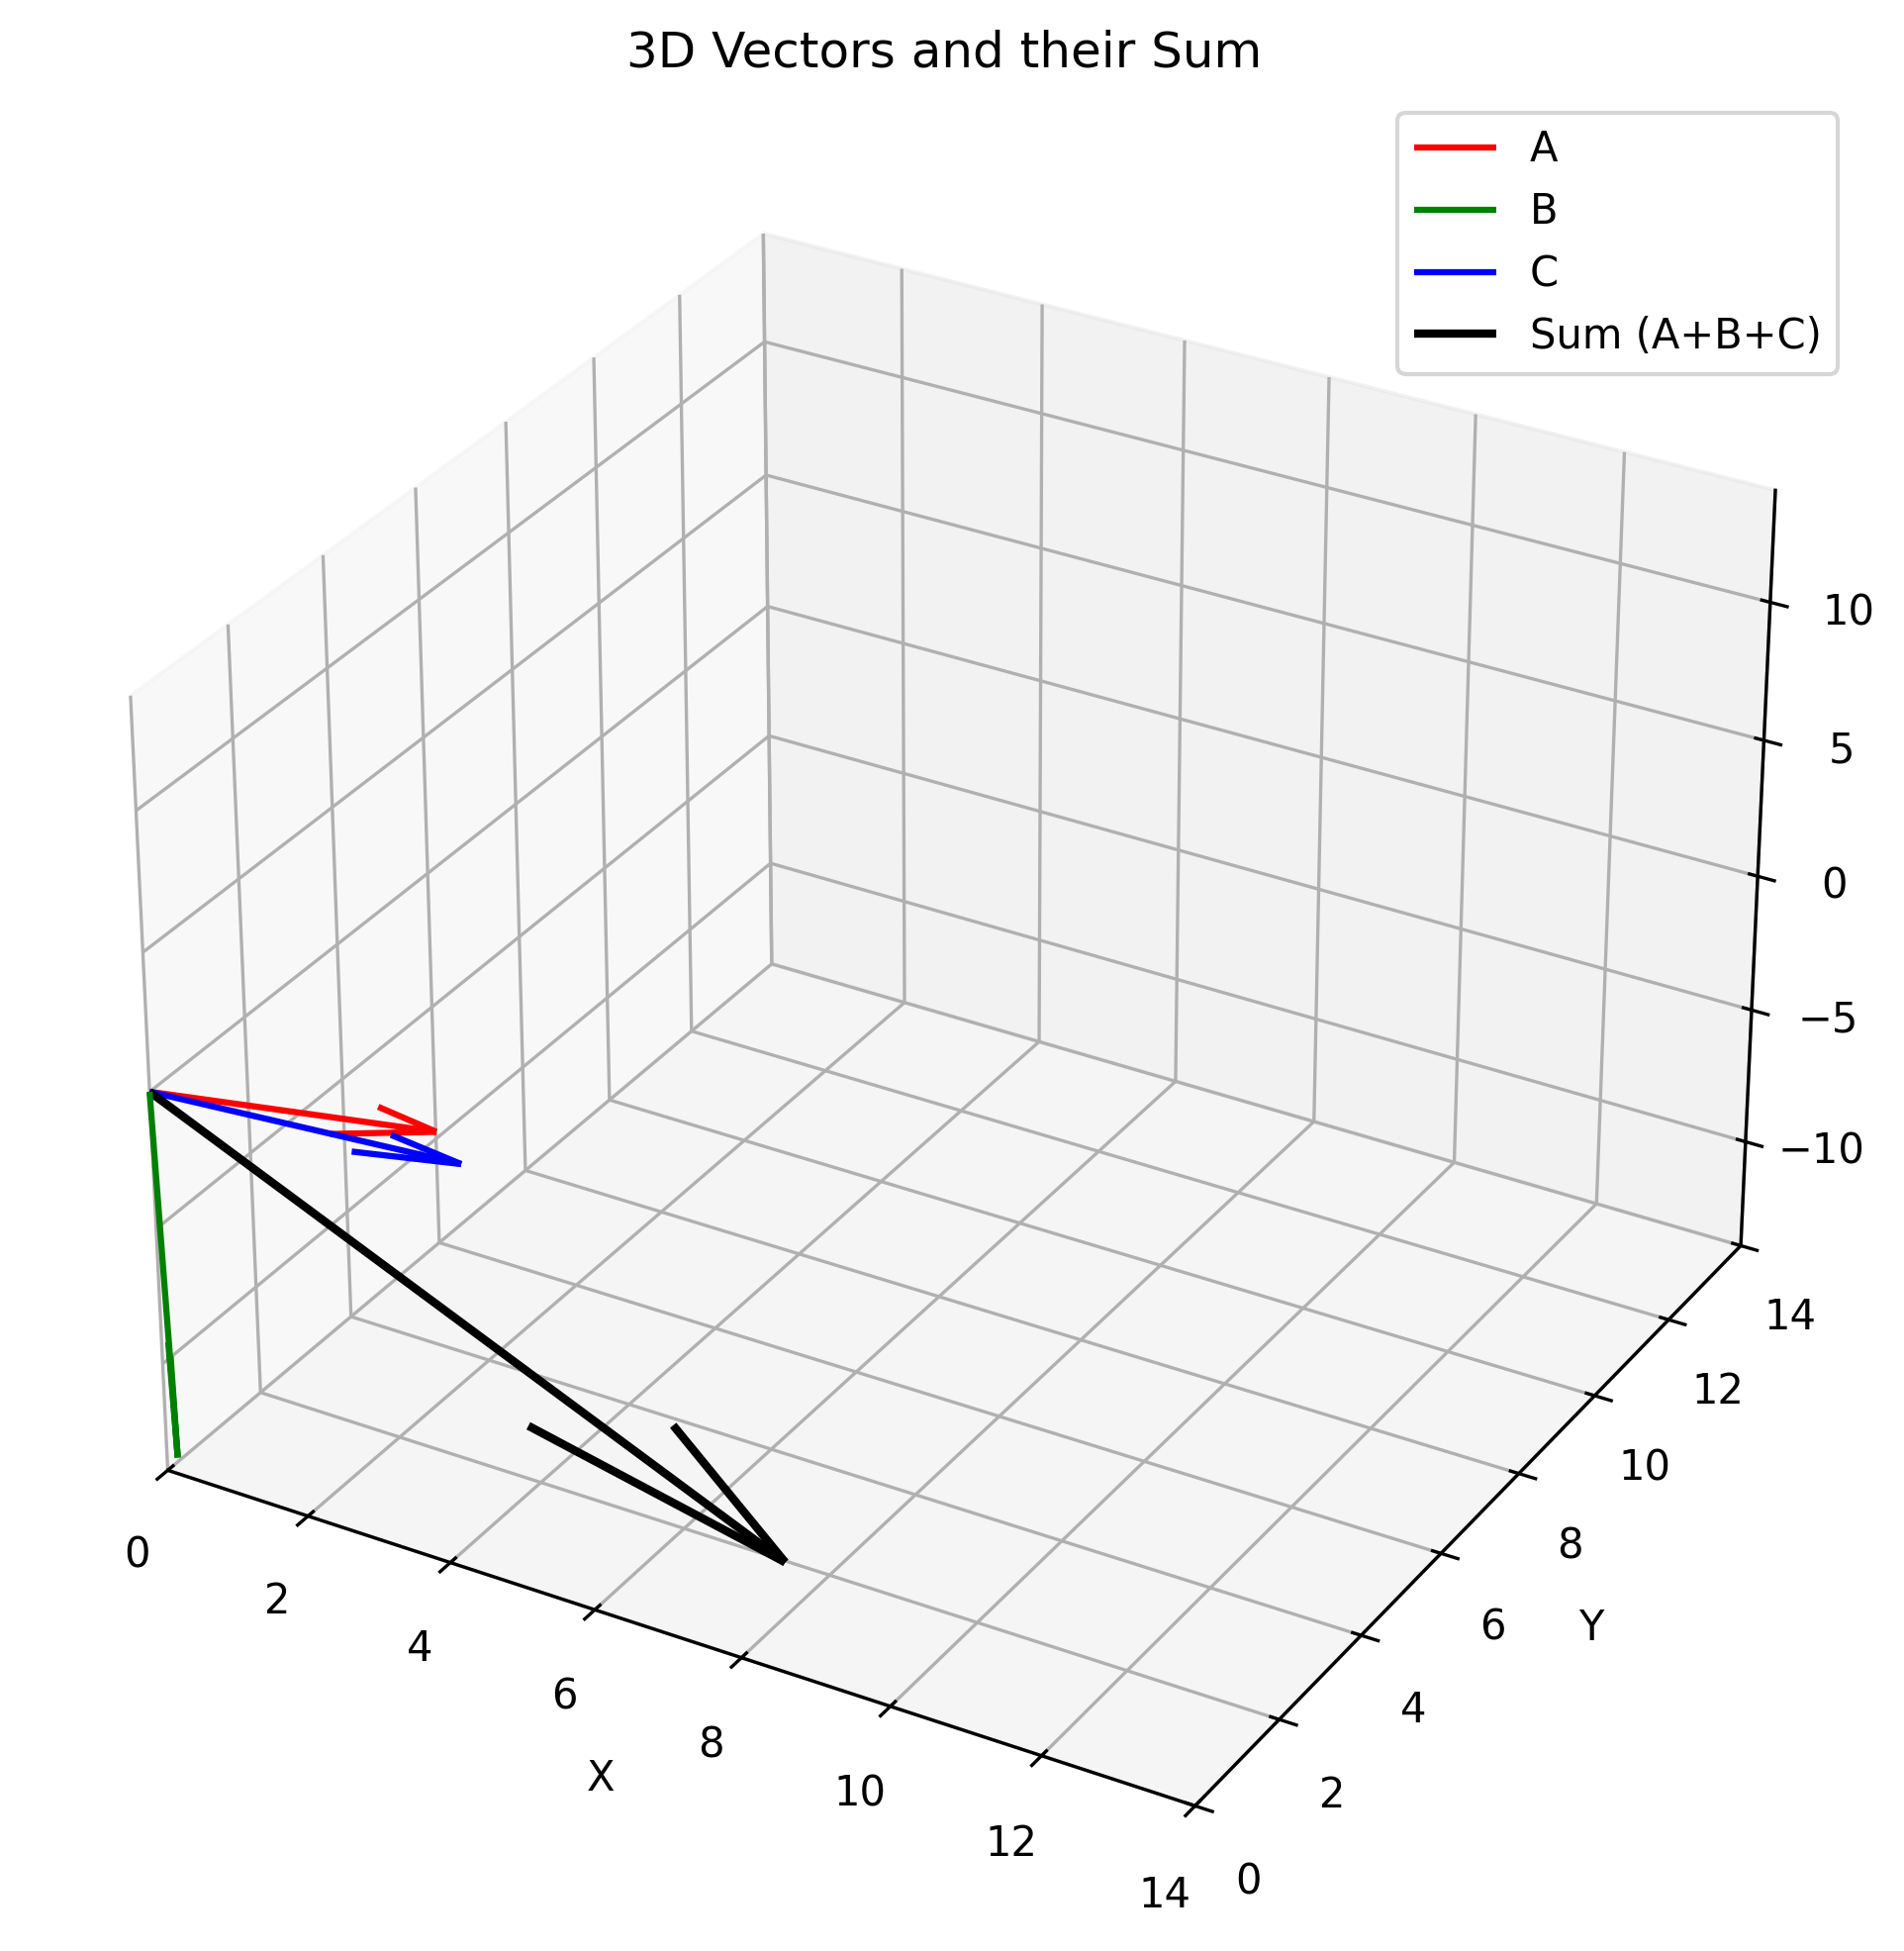
\includegraphics[height=0.5\textheight, keepaspectratio]{figs/Figure_1.png}
    \label{figure_1}
\end{figure}
 


\end{document}